%%%%%%%%%%%%%%%%%%%%%%%%%%%%%%%%%%%%%%%%%%%%%%%%%%%%%%%%%%%%%%%%
%
%  Template for homework of Introduction to Machine Learning.
%
%  Fill in your name, lecture number, lecture date and body
%  of homework as indicated below.
%
%%%%%%%%%%%%%%%%%%%%%%%%%%%%%%%%%%%%%%%%%%%%%%%%%%%%%%%%%%%%%%%%


\documentclass[11pt,letter,notitlepage]{article}

\usepackage[left=2cm, right=2cm, lines=45, top=0.8in, bottom=0.7in]{geometry}

\usepackage{fancyhdr}
\usepackage{fancybox}
\usepackage{graphicx}
\usepackage{pdfpages} 
\usepackage{enumitem}
\usepackage{algorithm}
\usepackage{algorithmic}

\usepackage{epstopdf}
\usepackage{subfigure}
\usepackage{threeparttable}


\renewcommand{\headrulewidth}{1.5pt}
\renewcommand{\footrulewidth}{1.5pt}
\newcommand\Loadedframemethod{TikZ}
\usepackage[framemethod=\Loadedframemethod]{mdframed}

\usepackage{amssymb,amsmath}
\usepackage{amsthm}
\usepackage{thmtools}

\setlength{\topmargin}{0pt}
\setlength{\textheight}{9in}
\setlength{\headheight}{0pt}

\setlength{\oddsidemargin}{0.25in}
\setlength{\textwidth}{6in}

%%%%%%%%%%%%%%%%%%%%%%%%
%%%%%% Define math operator %%%%%
%%%%%%%%%%%%%%%%%%%%%%%%
\DeclareMathOperator*{\argmin}{\bf argmin}
\DeclareMathOperator*{\relint}{\bf relint\,}
\DeclareMathOperator*{\dom}{\bf dom\,}
\DeclareMathOperator*{\intp}{\bf int\,}
%%%%%%%%%%%%%%%%%%%%%%%


\setlength{\topmargin}{0pt}
\setlength{\textheight}{9in}
\setlength{\headheight}{0pt}

\setlength{\oddsidemargin}{0.25in}
\setlength{\textwidth}{6in}
\pagestyle{fancy}
%%%%%%%%%%%%%%%%%%%%%%%%
%% Define the Exercise environment %%
%%%%%%%%%%%%%%%%%%%%%%%%
\mdtheorem[
topline=false,
rightline=false,
leftline=false,
bottomline=false,
leftmargin=-10,
rightmargin=-10
]{exercise}{\textbf{Exercise}}
%%%%%%%%%%%%%%%%%%%%%%%
%% End of the Exercise environment %%
%%%%%%%%%%%%%%%%%%%%%%%


%%%%%%%%%%%%%%%%%%%%%%%%
%% Define the Problem environment %%
%%%%%%%%%%%%%%%%%%%%%%%%
\mdtheorem[
topline=false,
rightline=false,
leftline=false,
bottomline=false,
leftmargin=-10,
rightmargin=-10
]{problem}{\textbf{Problem}}
%%%%%%%%%%%%%%%%%%%%%%%
%% End of the Exercise environment %%
%%%%%%%%%%%%%%%%%%%%%%%

%%%%%%%%%%%%%%%%%%%%%%%
%% Define the Solution Environment %%
%%%%%%%%%%%%%%%%%%%%%%%
\declaretheoremstyle
[
spaceabove=0pt, 
spacebelow=0pt, 
headfont=\normalfont\bfseries,
notefont=\mdseries, 
notebraces={(}{)}, 
headpunct={:\quad}, 
headindent={},
postheadspace={ }, 
postheadspace=4pt, 
bodyfont=\normalfont, 
qed=$\blacksquare$,
preheadhook={\begin{mdframed}[style=myframedstyle]\end{mdframed}},
	postfoothook={},
]{mystyle}

\declaretheorem[style=mystyle,title=Solution,numbered=no]{solution}
\mdfdefinestyle{myframedstyle}{%
	topline=false,
	rightline=false,
	leftline=false,
	bottomline=false,
	skipabove=-6ex,
	leftmargin=-10,
	rightmargin=-10}
%%%%%%%%%%%%%%%%%%%%%%%
%% End of the Solution environment %%
%%%%%%%%%%%%%%%%%%%%%%%

%% Homework info.
\newcommand{\posted}{\text{Nov. 16, 2021}}       			%%% FILL IN POST DATE HERE
\newcommand{\due}{\text{Nov. 29, 2021}} 			%%% FILL IN Due DATE HERE
\newcommand{\hwno}{\text{4}} 		           			%%% FILL IN LECTURE NUMBER HERE


%%%%%%%%%%%%%%%%%%%%
%% Put your information here %%
%%%%%%%%%%%%%%%%%%%
\newcommand{\name}{\text{San Zhang}}  	          			%%% FILL IN YOUR NAME HERE
\newcommand{\id}{\text{PBXXXXXXXX}}		       			%%% FILL IN YOUR ID HERE
%%%%%%%%%%%%%%%%%%%%
%% End of the student's info %%
%%%%%%%%%%%%%%%%%%%


\newcommand{\proj}[2]{\textbf{P}_{#2} (#1)}
\newcommand{\lspan}[1]{\textbf{span}  (#1)  }
\newcommand{\rank}[1]{ \textbf{rank}  (#1)  }
\newcommand{\RNum}[1]{\uppercase\expandafter{\romannumeral #1\relax}}
\DeclareMathOperator*{\cl}{\bf cl\,}
\DeclareMathOperator*{\bd}{\bf bd\,}
\DeclareMathOperator*{\conv}{\bf conv\,}
\DeclareMathOperator*{\epi}{\bf epi\,}


% \lhead{
% 	\textbf{\name}
% }
% \rhead{
% 	\textbf{\id}
% }
\chead{\textbf{
		Homework \hwno
}}




\begin{document}
\vspace*{-4\baselineskip}
\thispagestyle{empty}


\begin{center}
{\bf\large Introduction to Machine Learning}\\
{Spring 2021}\\
University of Science and Technology of China
\end{center}

\noindent
Lecturer: Jie Wang  			 %%% FILL IN LECTURER HERE
\hfill
Homework \hwno             			
\\
Posted: \posted
\hfill
Due: \due
% \\
% Name: \name             			
% \hfill
% ID: \id						
% \hfill

\noindent
\rule{\textwidth}{2pt}

\medskip





%%%%%%%%%%%%%%%%%%%%%%%%%%%%%%%%%%%%%%%%%%%%%%%%%%%%%%%%%%%%%%%%
%% BODY OF HOMEWORK GOES HERE
%%%%%%%%%%%%%%%%%%%%%%%%%%%%%%%%%%%%%%%%%%%%%%%%%%%%%%%%%%%%%%%%

\textbf{Notice, }to get the full credits, please present your solutions step by step.

\begin{exercise}[Convex Functions]
    \begin{enumerate}
        \item (Optional)
        For each of the following functions, determine whether it is convex. % and then show your conclusion.
        % \item Judgement questions.
        \begin{enumerate}
            \item
            $f(x)=x^2\log x$ on $\mathbb{R}_{++}$, where $\mathbb{R}_{++}=\{x\in\mathbb{R}:x>0\}$.
            \item
            $f(x_1,x_2)=x_1x_2$ on $\mathbb{R}^2$.
            \item
            $f(x_1,x_2)=\frac{x_1}{x_2}$ on $\mathbb{R}^2_{++}$, where $\mathbb{R}^2_{++}=\{ (x_1,x_2)\in\mathbb{R}^2:x_1,x_2>0\}$.
            \item
            $f(x_1,x_2)=\frac{x_1^2}{x_2}$ on $\mathbb{R}\times\mathbb{R}_{++}$.
            \item
            $f(x_1,x_2)=x_1^\alpha x_2^{1-\alpha}$ on $\mathbb{R}^2_{++}$, where $0\le\alpha\le 1$.
        \end{enumerate}
        \item
        Please show that the following functions are convex.
        \begin{enumerate}
            \item
            $ f(\mathbf{x})=\log \sum_{i=1}^n e^{x_i}$ 
            on $\dom f=\mathbb{R}^n$, where $x_i$ denotes the $i^{th}$ component of $\mathbf{x}$.
            
            \item
            $f(\mathbf{x})=\sum_{i=1}^k x_{[i]}$ on $\dom f=\mathbb{R}^n$, where $1\le k\le n$ and $x_{[i]}$ denotes the $i^{th}$ largest component of $\mathbf{x}$.
            
            \item The extended-value extension of the indicator function of a convex set $C\subseteq\mathbb{R}^n$, i.e.,
            \begin{align*}
                \Tilde{I}_c(\mathbf{x})=
                \begin{cases}
                    0,\hspace{4mm}\mathbf{x}\in C,\\
                    \infty,\hspace{3mm}\mathbf{x}\notin C.
                \end{cases}
            \end{align*}
            
            \item
            The negative entropy, i.e.,
            $$
            f(\mathbf{p})=\sum_{i=1}^n p_i\log p_i
            $$
            on $\dom f=\{ \mathbf{p}\in\mathbb{R}^n:0<p_i\le 1, \sum_{i=1}^n p_i=1\}$, where $p_i$ denotes the $i^{\text{th}}$ component of $\mathbf{p}$.
            
            \item
            The spectral norm, i.e.,
            $$
            f(\mathbf{X})=\|\mathbf{X}\|_2=\sigma_{\max}(\textbf{X})
            $$
            on $\dom f=\mathbb{R}^{m\times n}$,
            where $\sigma_{\max}$ denotes the largest singular value of $\textbf{X}$.
            
            \item
            $f(\mathbf{X})=\operatorname{tr} (\mathbf{X}^{-1})$ on $\dom f=\mathbb{S}_{++}^n$, where $\mathbb{S}_{++}^n$ is the space of all $n\times n$ real positive definite matrices.
            
        \end{enumerate}

    \item
    Please show that a continuously differentiable function $f$ is strongly convex with parameter $\mu>0$ if and only if 
    \begin{align*}
        f(\mathbf{y})\ge f(\mathbf{x})+\langle\nabla f(\mathbf{x}),\mathbf{y}-\mathbf{x}\rangle+\frac{\mu}{2}\|\mathbf{y}-\mathbf{x}\|_2^2,\quad \forall\, \mathbf{x},\mathbf{y}\in\mathbb{R}^n.
    \end{align*}
    \item
    Suppose that $f$ is twice continuously differentiable and strongly convex with parameter $\mu>0$. Please show that $\mu\leq \lambda_{\min}(\nabla^2 f(\mathbf{x}))$ for any $\mathbf{x}\in\mathbb{R}^n$, where $\lambda_{\min}(\nabla^2 f(\mathbf{x}))$ is the smallest eigenvalue of $\nabla^2 f(\mathbf{x})$.
    \item Suppose that $f:\mathbb{R}^n\rightarrow\mathbb{R}$ is twice continuously differentiable, and the gradient of $f$ is Lipschitz continuous, i.e.,
    \begin{align*}
        \|\nabla f(\mathbf{x})-\nabla f(\mathbf{y})\|_2\le L\|\mathbf{x}-\mathbf{y}\|_2,\quad \forall\,\mathbf{x},\mathbf{y}\in\mathbb{R}^n,
    \end{align*}
    where $L>0$ is the Lipschitz constant. Please show that $\lambda_{\max}(\nabla^2f(\mathbf{x}))\leq L$ for any $\mathbf{x}\in\mathbb{R}^n$, where $\lambda_{\max}(\nabla^2f(\mathbf{x}))$ is the largest eigenvalue of $\nabla^2 f(\mathbf{x})$.
    
    \item Consider the problem
    \begin{align}\label{prob:solution_of_conv}
        \min_{\textbf{x}\in\mathbb{R}^n}f(\mathbf{x}),
    \end{align}
    where $f:\mathbb{R}^n\rightarrow\mathbb{R}$ is  continuously differentiable and convex, and $\textbf{dom } f$ is closed.
    \begin{enumerate}
        \item
        Please show that the $\alpha$-sublevel set of $f$, i.e., $ C_\alpha=\{\mathbf{x}\in\textbf{dom }f:f(\mathbf{x})\leq \alpha\}
        $
        is closed.
        \item
        Please give an example to show that Problem (\ref{prob:solution_of_conv}) may be unsolvable even if $f$ is strictly convex. 
        \item 
        Suppose that $f$ can attain its minimum. Please show that the optimal set $\mathcal{C}=\{ \mathbf{y}:f(\mathbf{y})=\min_{\mathbf{x}} f(\mathbf{x})\}$ is closed and convex. Does this property still hold if $\textbf{dom }f$ is not closed?
        \item
        Suppose that $f$ is strongly convex with parameter $\mu>0$. Please show that Problem (\ref{prob:solution_of_conv}) admits a unique solution.
    \end{enumerate}
\end{enumerate}
    
\end{exercise}

\begin{solution}

\end{solution}

\newpage
\begin{exercise}[ Operations that Preserve Convexity ]
    \begin{enumerate}
        
        \item
        \begin{enumerate}
            \item Let $f:\mathbb{R}^m \rightarrow \left( -\infty,+\infty \right]$ be a given convex function, $\mathbf{A}\in \mathbb{R}^{m \times n}$ and $\mathbf{b} \in \mathbb{R}^m$. Please show that
        \begin{align*}
            F(\mathbf{x}) = f(\mathbf{Ax+b}),\quad\mathbf{x}\in\mathbb{R}^n.
        \end{align*}
        is convex.
        \item Let $f_i:\mathbb{R}^n \rightarrow \left(-\infty,+\infty \right],i=1,\dots,m$, be given convex functions. Please show that
        \begin{align*}
            F(\mathbf{x}) = \sum_{i=1}^m w_if_i(\mathbf{x})
        \end{align*}
        is convex, where $w_i \geq 0,\,i=1,\dots,m$.
        
        \item
            Let $f_i:\mathbb{R}^n \rightarrow \left(-\infty,+\infty \right]$ be given convex functions for $i \in I$, where $I$ is an arbitrary index set. Please show that the supremum
            \begin{align*}
                F(\mathbf{x}) = \sup_{i\in I}f_i(\mathbf{x})
            \end{align*}
            is convex.
            
        \end{enumerate}
        
        
        \item (Optional) Let $\mathbf{A}\in \mathbb{R}^{n\times m},\mathbf{x}_0\in \mathbb{R}^n$. The restriction of $f:\mathbb{R}^n\rightarrow\mathbb{R}$ to the affine set $\{\mathbf{Az}+\mathbf{x}_0|\mathbf{z}\in\mathbb{R}^m\}$ is defined as the function $F:\mathbb{R}^m\rightarrow\mathbb{R}$ with
        \begin{align*}
            F(\mathbf{z})=f(\mathbf{Az}+\mathbf{x}_0)
        \end{align*}
        on $\textbf{dom }F=\{\mathbf{z}|\mathbf{Az}+\mathbf{x}_0\in\textbf{dom }f\}$. Suppose $f$ is twice differentiable with a convex domain.
        \begin{enumerate}
            \item Show that $F$ is convex if and only if for all $\mathbf{z}\in\textbf{dom }F$, we have
            \begin{align*}
                \mathbf{A}^\top\nabla^2f(\mathbf{Az}+\mathbf{x}_0)\mathbf{A}\succeq 0.
            \end{align*}
            \item Suppose $\mathbf{B}\in\mathbb{R}^{p\times n}$ is a matrix whose nullspace is equal to the range of $\mathbf{A}$, i.e., $\mathbf{AB}=\mathbf{0}$ and $\operatorname{rank} (\mathbf{B})=n-\operatorname{rank}(\mathbf{A})$. Show that $F$ is convex if for all $\mathbf{z}\in\textbf{dom }F$, there exists a $\lambda\in\mathbb{R}$ such that
            \begin{align*}
                \nabla^2f(\mathbf{Az}+\mathbf{x}_0)+\lambda\mathbf{B}^\top\mathbf{B}\succeq 0.
            \end{align*}
            
            (\textbf{Hint:} you can use the result as follows. If $\mathbf{C}\in\mathbb{S}^n$ and $\mathbf{D}\in\mathbb{R}^{p\times n}$, then $\mathbf{x}^\top\mathbf{C}\mathbf{x}\geq 0$ for all $\mathbf{x}\in\mathcal{N}(\mathbf{D})$ if there exists a $\lambda$ such that $\mathbf{C}+\lambda\mathbf{D}^\top\mathbf{D}\succeq 0.$)
        \end{enumerate}
        
        
        \item (Optional) \begin{enumerate}
            
            
            \item
            Consider the function $f(\mathbf{X})=\lambda_{\max}(\mathbf{X})$, with $\dom\, f =\mathbb{S}^n$, where $\lambda_{\max}(\mathbf{X})$ is the largest eigenvalue of $\mathbf{X}$ and $\mathbb{S}^n$ is the set of $n\times n$ real symmetric matrices. Show that $f$ is a convex function.
            \item
            Let $f:\mathbb{R}^n\to\mathbb{R}$ be a convex function, with $\textbf{dom }f=\mathbb{R}^n$. Show that it can be represented as the pointwise supremum of a family of affine functions, i.e.,
            $$
            f(\mathbf{x})=\sup\{ g(\mathbf{x}): g\text{ is affine},g(\mathbf{z})\le f(\mathbf{z}) \text{ for all }\mathbf{z}\in\mathbb{R}^n\}.
            $$
        \end{enumerate}
        \item 
        Suppose that the training set is $\{(\mathbf{x}_i,y_i)\}_{i=1}^n$, where $\mathbf{x}_i\in\mathbb{R}^d$ is the $i^{th}$ data instance and $y_i\in\mathbb{R}$ is the corresponding label.
        Recall that Lasso is the regression problem:
        	\begin{align*}
            	\min_{\mathbf{w}}\,\frac{1}{2n}\|\mathbf{X}\mathbf{w}-\mathbf{y}\|_2^2+\lambda\|\mathbf{w}\|_1,
            \end{align*}
        	where $\mathbf{X}\in\mathbb{R}^{n\times d}$ with its $i^{th}$ row being $\mathbf{x}_i^{\top}$, $\mathbf{w} \in \mathbb{R}^d$, and $\lambda>0$ is the regularization parameter. Show that the objective function in the above problem is convex.
    	
    \end{enumerate}
\end{exercise}
\begin{solution}

\end{solution}


\newpage
\begin{exercise}[Subdifferentials]
    \begin{enumerate}
        \item Calculation of subdifferentials.
        \begin{enumerate}
            \item Let $H\subset\mathbb{R}^n$ be a hyperplane. The extended-value extension of its indicator function $I_H$ is
            \begin{align*}
                \Tilde{I}_H(\textbf{x})=\begin{cases}
                    0,&\textbf{x}\in H,\\
                    \infty,&\textbf{x}\not\in H.
                \end{cases}
            \end{align*}
            Find $\partial \Tilde{I}_H(\textbf{x})$.
            
            \item Let $f(\textbf{x})=\exp{\|\textbf{x}\|_1},\, \textbf{x}\in\mathbb{R}^n$. Find $\partial f(\textbf{x})$.
            
            \item Let $f(x)=\max\{0,x\},\,x\in\mathbb{R}$. Find $\partial f(x)$.
            
            \item For $\textbf{x}\in\mathbb{R}^n$, let $x_{[i]}$ be the $i^{th}$ largest component of $\textbf{x}$. Find the subdifferential of
            \begin{align*}
                f(\textbf{x})=\sum_{i=1}^k x_{[i]}.
            \end{align*}
            
            \item Let $f(\textbf{x})=\max\limits_{1\le i\le n} x_i,\, \textbf{x}\in\mathbb{R}^n$. Find $\partial f(\textbf{x})$.
            
            \item (Optional) Let
            \begin{align*}
                f(\textbf{x})=\left(\sum\limits_{i=1}^k x_i^2\right)^{\frac{1}{2}}+\left(\sum\limits_{i=k+1}^n x_i^2\right)^{\frac{1}{2}},\quad \textbf{x}\in\mathbb{R}^n,
            \end{align*}
            where $1\le k\le n-1$. Find $\partial f(\textbf{x})$.
            
            \item (Optional) Let $f(\textbf{X})=\|\textbf{X}\|_*$ be the trace norm of $\textbf{X}\in\mathbb{R}^{m\times n}$. Find $\partial f(\textbf{X})$.
            
        \end{enumerate}
        \item In Example 5 of Lecture 08, we got two forms of $\partial f(\textbf{x})$ by two approaches. Please show that they are the same, i.e., the following two sets are the same for $\forall \textbf{x}\in\mathbb{R}^n$.
        \begin{align*}
            &A_\textbf{x}=\{\textbf{y}\in\mathbb{R}^n:\langle\textbf{x},\textbf{y}\rangle=\|\textbf{x}\|_{\infty},\|\textbf{y}\|_1\le 1\}\\
            &B_\textbf{x}=\begin{cases}
                \{\textbf{y}\in\mathbb{R}^n:\|\textbf{y}\|\le1\},&\textbf{x}=\textbf{0},\\
                \{\textbf{y}\in\mathbb{R}^n:\sum_{i=1}^n \varepsilon_i y_i=1,\varepsilon_iy_i\ge 0,y_i=0\,\text{if}\,\varepsilon_i=0\},&\textbf{x}\neq \textbf{0},
            \end{cases}
        \end{align*}
        where $\varepsilon_i$ is defined as
        \begin{align*}
            \varepsilon_i=\begin{cases}
                1,&x_i=\|\textbf{x}\|_\infty,\\
                0,&|x_i|<\|\textbf{x}\|_\infty,\\
                -1,&x_i=-\|\mathbf{x}\|_\infty.
            \end{cases}
        \end{align*}
    \end{enumerate}
\end{exercise}
\begin{solution}

\end{solution}

\newpage
\begin{exercise}[Proximal Gradient]
Consider the following convex optimization problem
\begin{align}\label{prob:ex2}
    \min_\textbf{x}\, &F(\textbf{x})\\
    \nonumber\text{s.t.} &\textbf{x}\in D
\end{align}
where $F:\mathbb{R}^n\rightarrow\overline{\mathbb{R}}$ is a proper convex function and $D\subseteq\mathbb{R}^n$
is a nonempty convex set with $D\subseteq\dom F$. Suppose that the problem (\ref{prob:ex2}) is solvable, and {\bf we do not require the differentiability of $F$}.
\begin{enumerate}
    \item If $\textbf{x}\in\intp(\dom F) \cap D$ and there exists a $\textbf{g}\in\partial F(\textbf{x})$ such that
    \begin{align*}
        \langle \textbf{g},\textbf{y}-\textbf{x} \rangle\ge 0,\, \forall\, \textbf{y}\in D,
    \end{align*}
    show that $\textbf{x}$ is optimal.
    
    \item (Optional) If $\textbf{x}\in\intp(\dom F)$ and $\textbf{x}$ is optimal, show that $\textbf{x}\in D$ and there exists a $\textbf{g}\in\partial F(\textbf{x})$ such that
    \begin{align*}
        \langle \textbf{g},\textbf{y}-\textbf{x} \rangle\ge 0,\, \forall\, \textbf{y}\in D.
    \end{align*}
    
    \item Please give an example to show that $\partial F(\textbf{x})$ can be empty.
    
    \item If $\textbf{x}^*$ is an interior point of $D$, show that
    \begin{align*}
        \mathbf{x}^*\in\argmin_{\mathbf{x}\in D}\,F(\mathbf{x})\Leftrightarrow 0\in\partial F(\mathbf{x}^*).
    \end{align*}
    You can use the conclusion of Problems 1 and 2.
\end{enumerate}
In many cases, the function $F$ can be decomposed into $F=f+g$,
where $g:\mathbb{R}^n\to\overline{\mathbb{R}}$ is a continuous convex function, and $f:\mathbb{R}^n\to\mathbb{R}$ is a convex and continuously differentiable function, whose gradient is Lipschitz continuous with the constant $L$.
We can use ISTA, which has been introduced in Lecture 08, to find $\min\limits_{\textbf{x}\in\mathbb{R}^n} F(\textbf{x})$.

\begin{enumerate}[resume]
    \item For a \textbf{given} point $\textbf{x}_c$, we consider the following quadratic approximation of $F$:
    \begin{align*}
       Q(\mathbf{x};\mathbf{x}_c)=f(\mathbf{x}_c)+\langle\nabla f(\mathbf{x}_c),\mathbf{x}-\mathbf{x}_c\rangle+\frac{L}{2}\|\mathbf{x}-\mathbf{x}_c\|^2+g(\mathbf{x}).
    \end{align*}
    Please show that it always admits a unique minimizer
    \begin{align*}
       p(\mathbf{x}_c)=&\argmin_{\textbf{x}\in\mathbb{R}^n}Q(\mathbf{x};\mathbf{x}_c).
    \end{align*}
    
    \item (Optional) We can think of the update step of ISTA, i.e.,  $\textbf{x}^+=p(\textbf{x})$, as two steps:
    \begin{enumerate}
        \item Take a step in the opposite direction of the gradient of $f$ at $\textbf{x}$, i.e., 
        \begin{align*}
             \textbf{z}=\textbf{x}-\frac{1}{L}\nabla f(\textbf{x}).
        \end{align*}
        
        \item Project $\textbf{z}$ on some set $C$, i.e.,
        \begin{align*}
            \textbf{x}^+=p(\textbf{x})=\Pi_C(\textbf{x}).
        \end{align*}
        
    \end{enumerate}
    Find the set $C$. Is it closed, open or neither? Is it convex or not?
    
    \item Consider the Lasso problem
    \begin{align*}
        \min_{\textbf{w}\in\mathbb{R}^n} \frac{1}{n} \|\textbf{y}-\textbf{X}\textbf{w}\|_2^2+\lambda\|\textbf{w}\|_1.
    \end{align*}
    Suppose that $\hat{\textbf{w}}$ solves the problem. Write down the optimality condition at $\hat{\textbf{w}}$.
    
    \item If we use ISTA to solve the Lasso problem, show that
    \begin{align*}
        w_i^+=
        \begin{cases}
            z_i+\dfrac{\lambda}{L},\,&\text{if}\,z_i<-\dfrac{\lambda}{L},\\
            0,\,&\text{if}\,|z_i|\le\dfrac{\lambda}{L},\\
            z_i-\dfrac{\lambda}{L},\,&\text{if}\,z_i>\dfrac{\lambda}{L},
        \end{cases}
    \end{align*}
    where $\textbf{z}=\textbf{w}_k-\dfrac{2}{Ln}\textbf{X}^\top(\textbf{X}\textbf{w}_k-\textbf{y})$.
    
    \item (Optional) Consider the convex optimization problem
    \begin{align}\label{prob:indicator}
        \min_{\textbf{x}\in\mathbb{R}^n} f(\textbf{x})+\Tilde{I}_D(\textbf{x}),
    \end{align}
    where $D\subseteq\mathbb{R}^n$ is a closed convex set and $\Tilde{I}_D(\textbf{x})$ is the extended-value extension of its indicator function $I_D(\textbf{x})$. 
    \begin{enumerate}
        \item Write down the optimality condition and the proximal operator of Problem (\ref{prob:indicator}).
        \item Find the relationship between (\ref{prob:indicator}) and the constrained optimization problem
        \begin{align*}
        \min_{\textbf{x}\in D} f(\textbf{x}).
        \end{align*}
    \end{enumerate}
     
    
    \item (Optional) Write down the proximal operator of the following convex optimization problems.
    \begin{enumerate}
        \item 
        \begin{align*}
        \min_{w\in\mathbb{R}^n} \frac{1}{n}\|\textbf{y}-\textbf{X}\textbf{w}\|_2^2+\lambda_1 \|\textbf{w}\|_1+\lambda_2 I_{\mathbb{R}^n_+}(\textbf{w}),
        \end{align*}
        
        \item 
        \begin{align*}
        \min_{w\in\mathbb{R}^n} \frac{1}{n}\|\textbf{y}-\textbf{X}\textbf{w}\|_2^2+\lambda \left[\left(\sum\limits_{i=1}^k x_i^2\right)^{\frac{1}{2}}+\left(\sum\limits_{i=k+1}^n x_i^2\right)^{\frac{1}{2}}\right].
        \end{align*}
    \end{enumerate}
    
\end{enumerate}

\end{exercise}
\begin{solution}

\end{solution}

\newpage
\begin{exercise}[Projected Gradient Descent (Optional)]
    Consider the following problem 
    \begin{align}\label{prob:sc_min}
        \min_{x\in D}f(x),
    \end{align}
    where $f:\mathbb{R}^{n} \to \overline{\mathbb{R}}$ is proper, continuously differentiable and strongly convex with convexity parameter $\mu>0$. We assume that the gradient of $f$ is Lipschitz with a constant $L>0$. 
    \par A commonly used approach to solve the constrained optimization problem (\ref{prob:sc_min}) is the so-called \emph{projected gradient descent}, in which each iteration improves the current estimation $\mathbf{x}_k$ of the optimum by
    \begin{align*}
        \mathbf{x}_{k+1}=\Pi_{D}(\textbf{x}_k-\alpha\nabla f(\textbf{x}_k)),
    \end{align*}
    where $\alpha>0$ is the step size.
    \begin{enumerate}
        \item Show that
        \begin{align*}
            f(\mathbf{y})\ge f(\mathbf{x})-\frac{1}{2\mu}\|\nabla f(\mathbf{x})\|_2^2, \,\forall\, \mathbf{x},\mathbf{y} \in D.
        \end{align*}
        \item Consider the problem (\ref{prob:sc_min}) and the sequence generated by the \emph{projected gradient descent} algorithm. Suppose that $\mathbf{x}^*$ is the solution to the problem (\ref{prob:sc_min}).
        \begin{enumerate}
            \item Find the range of $\alpha$ such that the function values $f(\mathbf{x}_k)$ converge linearly to $f(\mathbf{x}^*)$.
            \item When does the (projected) gradient descent always achieve the optimal solution in one iteration wherever the intial point $\mathbf{x}_0$ is?
        \end{enumerate}
    \end{enumerate}
\end{exercise}


\begin{solution}

\end{solution}

\newpage
\begin{exercise}[\cite{beck2009fast} ISTA with Backtracking]\label{exercise:ISTA-backtracking}
Suppose that we would like to apply ISTA to solve the convex optimization problem
\begin{align}\label{prob:f+g}
    \min_{\textbf{x}\in\mathbb{R}^n} F(\textbf{x})=f(\textbf{x})+g(\textbf{x}),
\end{align}
where $g:\mathbb{R}^n\to\overline{\mathbb{R}}$ is a continuous convex function, and $f:\mathbb{R}^n\to\mathbb{R}$ is a convex and continuously differentiable function, whose gradient is Lipschitz continuous with the constant $L$. We assume that Problem (\ref{prob:f+g}) is solvable, i.e., there exists $\textbf{x}^*$ such that 
\begin{align*}
    F(\textbf{x}^*)=F^*=\min_{\textbf{x}\in\mathbb{R}^n} F(
    \textbf{x}).
\end{align*}
In practice, however, a possible drawback of ISTA is that the Lipschitz constant $L$ is not always known or computable. For instance, if $f(\textbf{x})=\|\textbf{A}\textbf{x}-\textbf{b}\|_2^2$, the Lipschitz constant for $\nabla f$ depends on $\lambda_{\rm max}(\textbf{A}^\top\textbf{A})$, which is not always easily computable for large-scale problems. To tackle this problem, we always equip ISTA with the backtracking stepsize rule as shown in Algorithm \ref{alg:ISTA-back}. 
\par Note that in Algorithm \ref{alg:ISTA-back}, $Q_L$ and $p_L$ are defined as
\begin{align*}
    &Q_{L}(\textbf{x};\textbf{x}_c)=f(\textbf{x}_c)+\langle\nabla f(\textbf{x}_c),\textbf{x}-\textbf{x}_c\rangle+\frac{L}{2}\|\textbf{x}-\textbf{x}_c\|_2^2+g(\textbf{x})\\
    &p_L(\textbf{x}_c)=\argmin_{\textbf{x}\in\mathbb{R}^n} Q_L(\textbf{x};\textbf{x}_c).
\end{align*}

\begin{algorithm}[H]
	\caption{ISTA with Backtracking}\label{alg:ISTA-back}
	\begin{algorithmic}[1]
		\STATE {\bf Input:} An initial point $\mathbf{x}_0$, an initial  constant $L_0>0$, a threshold $\eta>1$, and $k=1$.
		\WHILE{the {\it termination condition} does not hold}
		    \STATE Find the smallest non-negative integer $i_k$ such that with $\Tilde{L}=\eta^{i_k}L_{k-1}$
		    \begin{align}\label{eqn:FQ}
		        F(p_{\Tilde{L}}(\textbf{x}_{k-1}))\le Q_{\Tilde{L}}(p_{\Tilde{L}}(\textbf{x}_{k-1});\textbf{x}_{k-1}).
		    \end{align}
		    \STATE $L_k\leftarrow \eta^{i_k}L_{k-1}$, $\textbf{x}_k\leftarrow p_{L_k}(\textbf{x}_{k-1})$,
		    \STATE $k \leftarrow k+1$,
		\ENDWHILE
		
	\end{algorithmic}
\end{algorithm}

\begin{enumerate}
    \item Show that the sequence $\{F(\textbf{x}_k)\}$ produced by Algorithm \ref{alg:ISTA-back} is non-increasing.
    
    \item Show that Inequality (\ref{eqn:FQ}) is satisfied for any $\Tilde{L}\ge L$, where $L$ is the Lipschitz constant of $\nabla f$, thus showing that for Algorithm \ref{alg:ISTA-back} one has $L_k\le \eta L$ for every $k\ge 1$.
    
    \item Let $\{\textbf{x}_k\}$ be the sequence generated by Algorithm \ref{alg:ISTA-back}. Show that for any $k\ge 1$ we have
    \begin{align*}
        F(\textbf{x}_k)-F(\textbf{x}^*)\le \frac{\eta L \|\textbf{x}_0-\textbf{x}^*\|_2^2}{2k},\,\forall \textbf{x}^*\in \argmin_{\textbf{x}\in\mathbb{R}^n} F(\textbf{x}).
    \end{align*}
    The above result means that the number of iterations of Algorithm \ref{alg:ISTA-back} required to obtain an $\varepsilon$-optimal solution, i.e., an $\hat{\textbf{x}}$ such that $F(\hat{\textbf{x}})-F(\textbf{x}^*)\le \varepsilon$, is at most
    \begin{align*}
        \left\lceil \frac{\eta L \|\textbf{x}_0-\textbf{x}^*\|_2^2}{2\varepsilon} \right\rceil.
    \end{align*}
\end{enumerate}


\end{exercise}
\begin{solution}

\end{solution}

\newpage
\begin{exercise}[Programming Exercise: Handwritten Digits Recognition]
    MNIST is a widely used data set---which consists of grey images of handwritten digits---in machine learning and pattern recognition. The training set and the testing set have 60000 and 10000 images, respectively. We show ten images in MNIST in Figure (a).
    
    In this exercise, we would like to predict the label of a given handwritten image. Notice that, the labels of the images in the training set come for granted. For example, given an image from the training set with a handwritten digit ``$7$" in it, we know the number (the label) in the image is $7$. Our task is to predict the number in a handwritten image outside of the training set.
    
    To do so, we first transform the $28\times28$ gray images in the training set into a set of $784$-dimensional column vectors, and then we put them together to construct the input feature matrix $\textbf{X} \in \mathbb{R}^{n\times d}$, where $n=784$ and $d=60000$. We also provide you labels of all images in the training set. Then, we randomly choose an image in the testing set and transform it into a column vector in the same way as the corresponding response vector $\textbf{y}\in \mathbb{R}^n$. We show this image in Figure (b).
    
    % A toy example is illustrated in Figure (a) and Figure (b).
    To predict the label of the response vector, we use Lasso to fit this data. Please follow the instructions step by step. You can use your favorite programming language.
\end{exercise}
    
 \begin{figure}[htp]
  \centering
  \subfigure[Ten images in the training set.]{
    \label{fig:subfig:1} %% label for first subfigure
    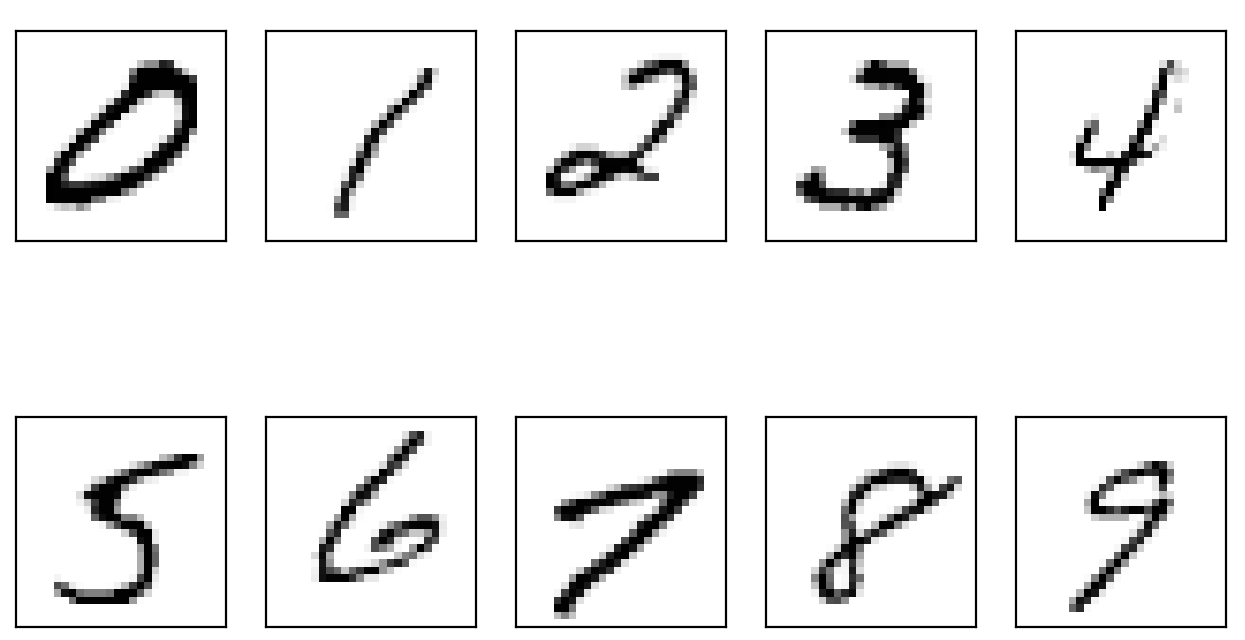
\includegraphics[width=3.0in]{HW4/figures/0_9.png}}
  \hspace{1in}
  \subfigure[The image we choose from the testing set. ]{
    \label{fig:subfig:2} %% label for second subfigure
    
\includegraphics[width=1.55in]{HW4/figures/4.png}}
  \label{fig:subfig} %% label for entire figure
\end{figure} 

    
    \begin{enumerate}
        \item We first normalize the data matrix $\mathbf{X}$ and the response vector $\mathbf{y}$, such that each entries are within $[0,1]$. Specifically, let 
        \begin{align*}
            \mathbf{Z}= \mathbf{X}/255,\mathbf{h}=\mathbf{y}/255.
        \end{align*}
        Then, Lasso takes the form of
        \begin{align}\label{prob:lsm2}
          \min_{\textbf{u}}F(\textbf{u}) = \frac{1}{n}\|\textbf{h}-\textbf{Z}\textbf{u}\|_2^2+\lambda\|\textbf{u}\|_1,
        \end{align}
        where $\textbf{u}\in\mathbb{R}^{d}$. Let $f(\textbf{u})=\frac{1}{n}\|\textbf{ h}-\textbf{Z}\textbf{u}\|_2^2$ and $g(\textbf{u})=\lambda\|\textbf{u}\|_1$.
        \item
        Please find the Lipschitz constants of  $\nabla f(\textbf{u})$ and write down the corresponding quadratic approximation function of $F(\textbf{u})$.
        \item From 0.002 to 0.2, uniformly pick out 100 different $\lambda$s and then implement the ISTA algorithm in \textbf{Exercise} \ref{exercise:ISTA-backtracking} to solve Problem (\ref{prob:lsm2}), with different $\lambda$s. Terminate the iteration after 2000 steps and denote the $\textbf{u}_{2000}$ by $\textbf{u}'$. Please plot scatter diagrams of $f(\textbf{u}')$ versus $\lambda$, $g(\textbf{u}')$ versus $\lambda$ and $F(\textbf{u}')$ versus $\lambda$, respectively. Besides, please plot a scatter diagram of the ration of nonzero elements in $\textbf{u}'$ versus $\lambda$.
    
        \item Please explain the practical meaning of the zero elements and nonzero elements in $\textbf{u}'$ and give your prediction about the digit in $\textbf{y}$ using our provided labels.
        \item (Optional) There exists a threshold value, which satisfies  that if $\lambda$ exceeds this value, $\textbf{u}'=\textbf{0}$. Please find this threshold in theory.
    \end{enumerate}

\begin{solution}

\end{solution}

\newpage
\bibliography{refs}
\bibliographystyle{abbrv}

%%%%%%%%%%%%%%%%%%%%%%%%%%%%%%%%%%%%%%%%%%%%%%%%%%%%%%%%%%%%%%%%

\end{document}
